\documentclass[12pt]{article}
\usepackage{amsthm,amssymb,amsfonts,amsmath,amstext,systeme}
\usepackage{graphicx,float}

\marginparwidth 0pt
\oddsidemargin -1.2 truecm
\evensidemargin  0pt 
\marginparsep 0pt
\topmargin -2.2truecm
\linespread{1}
\textheight 25.8 truecm
\textwidth 18.5 truecm
\newenvironment{remark}{\noindent{\bf Remark }}{\vspace{0mm}}
\newenvironment{remarks}{\noindent{\bf Remarks }}{\vspace{0mm}}
\newenvironment{question}{\noindent{\bf Question }}{\vspace{0mm}}
\newenvironment{questions}{\noindent{\bf Questions }}{\vspace{0mm}}
\newenvironment{note}{\noindent{\bf Note }}{\vspace{0mm}}
\newenvironment{summary}{\noindent{\bf Summary }}{\vspace{0mm}}
\newenvironment{back}{\noindent{\bf Background}}{\vspace{0mm}}
\newenvironment{conclude}{\noindent{\bf Conclusion}}{\vspace{0mm}}
\newenvironment{concludes}{\noindent{\bf Conclusions}}{\vspace{0mm}}
\newenvironment{dill}{\noindent{\bf Description of Dill's model}}{\vspace{0mm}}
\newenvironment{maths}{\noindent{\bf Mathematics needed}}{\vspace{0mm}}
\newenvironment{inst}{\noindent{\bf Instructions}}{\vspace{0mm}}
\newenvironment{notes}{\noindent{\bf Notes }}{\vspace{0mm}}
\newenvironment{theorem}{\noindent{\bf Theorem }}{\vspace{0mm}}
\newenvironment{example}{\noindent{\bf Example }}{\vspace{0mm}}
\newenvironment{examples}{\noindent{\bf Examples }}{\vspace{0mm}}
\newenvironment{topics}{\noindent{\bf Topics}}{\vspace{0mm}}
\newenvironment{outcomes}{\noindent{\bf Expected Learning Outcomes}}{\vspace{0mm}}
\newenvironment{lemma}{\noindent{\bf Lemma }}{\vspace{0mm}}
\newenvironment{solution}{\noindent{\it Solution}}{\vspace{2mm}}
\newcommand{\ds}{\displaystyle}
\newcommand{\un}{\underline}
\newcommand{\bs}{\boldsymbol}

\begin{document}

\baselineskip 18 pt
\begin{center}
	{\large \bf HKDSE MATH M2 2014}\\
	\vspace{2 mm}

\end{center}
\vspace{0.05cm}

\begin{enumerate}
	\item \textbf{HKDSE Math M2 2014 Q1}\\
	In the expansion of $(1-4x)^2(1+x)^n$, the coefficient of $x$ is 1.
	\begin{enumerate}
		\item [(a)]Find the value of $n$. 
		\item [(b)]Find the coefficient of $x^2$. 
	\end{enumerate}
	(4 marks)

	\item \textbf{HKDSE Math M2 2014 Q2}\\
	Consider the curve $C : y = x^3-3x$. 
	\begin{enumerate}
		\item [(a)]Find $\displaystyle\frac{dy}{dx}$ from first principles. 
		\item [(b)]Find the range of $x$ where $C$ is decreasing.
	\end{enumerate}
	(5 marks)

	\item \textbf{HKDSE Math M2 2014 Q3}\\
	Find the equation of tangent to the curve $x\ln{y} + y = 2$ at the point where the curve cuts the $y$-axis.\\
	(5 marks)

	\item \textbf{HKDSE Math M2 2014 Q4}\\
	Let $x = 2y + \sin{y}$. Find $\displaystyle\frac{d^2y}{dx^2}$ in terms of $y$.\\
	(3 marks)

	\item \textbf{HKDSE Math M2 2014 Q5}
	\begin{enumerate}
		\item [(a)]Find $\displaystyle\int \frac{dx}{\sqrt{9-x}}$, where $x < 9$. 
		\item [(b)]Using integration by substitution, find $\displaystyle\int \frac{dx}{\sqrt{9-x^2}}$, where $-3 < x < 3$.
	\end{enumerate}
	(6 marks)

	\item \textbf{HKDSE Math M2 2014 Q6}
	\begin{enumerate}
		\item [(a)]Find $\displaystyle\int xe^{-x}\,dx$. 
		\item [(b)]	Figure 1 shows the shaded region bounded by the curve $y = xe^{-x}$ and the straight line $y = \displaystyle\frac{x}{e}$. Find the area of the shaded region.
		\begin{figure}[H]
			\centering
			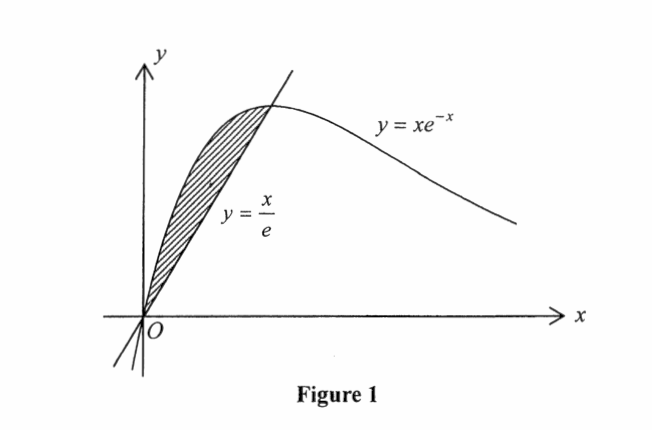
\includegraphics[width = .5\linewidth]{2014Figure1}
		\end{figure}

	\end{enumerate}
	(6 marks)

	\item \textbf{HKDSE Math M2 2014 Q7}\\
	Let $A = \begin{pmatrix}
		1&0&1\\
		0&2&0\\
		1&0&1\\
	\end{pmatrix}$.
	\begin{enumerate}
		\item [(a)]Prove, by mathematical induction, that for all positive integers $n$, $A^{n+1} = 2^nA$. 
		\item [(b)]Using the result of (a), Willy proceeds in the following way:\\
			$A^2 = 2A$\\
			$A^2 A^{-1}= 2AA^{-1}$\\
			$A = 2I$\\
			Explain why Willy arrives at a wrong conclusion.
	\end{enumerate}
	(7 marks)

	\item \textbf{HKDSE Math M2 2014 Q8}\\
	Let 
	$\overrightarrow{OP} = -\textbf{i} +2 \textbf{j} +2\textbf {k}$, 
	$\overrightarrow{OQ} = \textbf{i} - \textbf{j} +2\textbf {k}$ and 
	$\overrightarrow{OR} = 2\textbf{i} -3 \textbf{j} +6\textbf {k}$. 
	\begin{enumerate}
		\item [(a)]Find $\overrightarrow{OP} \times \overrightarrow{OQ}$. \\
		Hence find the volume of tetrahedron $OPQR$. 
		\item [(b)]Find the acute angle between the plane $OPQ$ and the line $OR$, correct to the nearest $0.1^\circ$.
	\end{enumerate}
	(8 marks)

	\item \textbf{HKDSE Math M2 2014 Q9}
	\begin{enumerate}
		\item [(a)]Solve the system of linear equations $\left\{
		\begin{matrix}
			x & + & y & + & z & = & 100\\
			x & + & 6y& + &10z& = & 200\\
		\end{matrix}\right.$
		\item [(b)]In a store, the prices of each of small, medium and large marbles are \$0.5, \$3 and \$5 respectively. Aubrey plans to spend all \$100 for exactly 100 marbles, which include $m$ small marbles, $n$ medium marbles and $k$ large marbles.\\
		Aubrey claims that there is only one set of combination of $m$, $n$ and $k$. Do you agree? Explain your answer.
	\end{enumerate}
	(6 marks)

	\item \textbf{HKDSE Math M2 2014 Q10}\\
	Thomas has a bookcase of dimensions 100 cm $\times$ 24 cm $\times$ 192 cm at the corner in his room. He wants to hang a decoration on the wall above the bookcase. Therefore, he finds a ladder to climb up. Initially, the ladder touches the wall, the edge of the top of the bookcase and the floor at the same time. Let rectangle $ABCD$ be the side-view of the bookcase and $HK$ be the side-view of the ladder, so that $AB = 24$ cm and $BC = 192$ cm (see Figure 2). Let $\angle HKD = \theta$. 
	\begin{figure}[H]
		\centering
		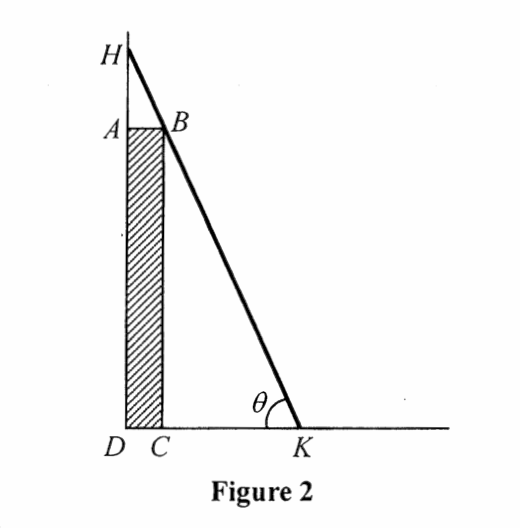
\includegraphics{2014Figure2}
	\end{figure}
	\begin{enumerate}
		\item [(a)]Find the length of $HK$ in terms of $\theta$. \\(1 marks)
		\item [(b)]Prove that the shortest length of the ladder is $120\sqrt{5}$ cm. \\(5 marks)
		\item [(c)]
		Suppose the length of the ladder is 270 cm. Suddenly, the ladder slides down so that the end of the ladder, $K$, moves towards $E$ (see Figure 3). The ladder touches the edge of the top of the bookcase and the floor at the same time. Let $x$ cm and $y$ cm be the horizontal distances from $H$ and $K$ respectively to the wall.
		\begin{figure}[H]
			\centering
			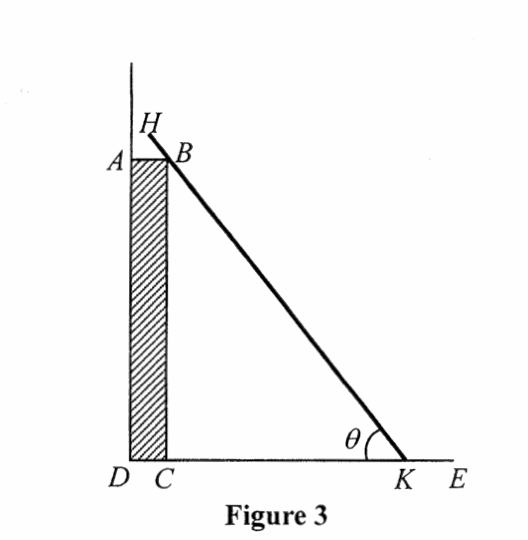
\includegraphics[width = .5\linewidth]{2014Figure3}
		\end{figure}
		\begin{enumerate}
			\item [(i)]When $CK = 160$ cm, the rate of change of $\theta$ is $-0.1$ rad s$^{-1}$. Find the rate of change of $x$ at this moment, correct to 4 significant figures. 
			\item [(ii)]Thomas claims that $K$ is moving towards $E$ at a speed faster than the horizontal speed $H$ is leaving the wall. Do you agree? Explain your answer.
		\end{enumerate}
		(6 marks)
	\end{enumerate}

	\item \textbf{HKDSE Math M2 2014 Q11}\\
	In Figure 4, $C$ and $D$ are points on $OB$ and $OA$ respectively such that $AD : DO = OC : CB = t : 1-t$, where $0 < t < 1$. $BD$ and $AC$ intersect at $E$ such that $AE : EC = m : 1 $ and $BE : ED = n : 1 $, where $m$ and $n$ are positive. Let $\overrightarrow{OA} = \textbf{a}$ and $\overrightarrow{OB} = \textbf{b}$. 
	\begin{figure}[H]
		\centering
		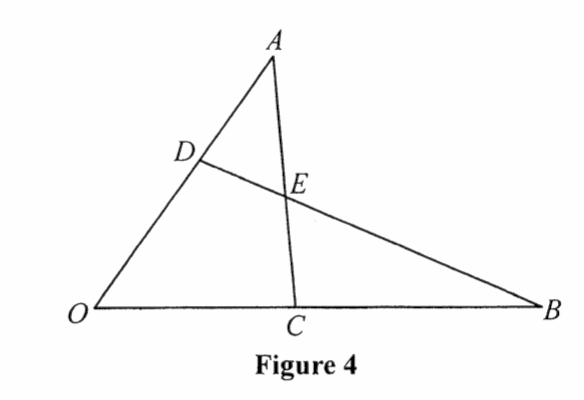
\includegraphics[width = .5\linewidth]{2014Figure4}
	\end{figure}
	\begin{enumerate}
		\item [(a)]
		\begin{enumerate}
			\item [(i)]By considering $\triangle OAC$, express $\overrightarrow{OE}$ in terms of $m$, $t$, $\textbf{a}$ and $\textbf{b}$.
			\item [(ii)]By considering $\triangle OBD$, express $\overrightarrow{OE}$ in terms of $n$, $t$, $\textbf{a}$ and $\textbf{b}$.
			\item [(iii)]Show that $\displaystyle m = \frac{t}{(1-t)^2}$ and $\displaystyle n = \frac{1-t}{t^2}$. 
			\item [(iv)]Chris claims that \\
				"if $m = n$, then $E$ is the centroid of $\triangle OAB$ ".\\
				Do you agree? Explain your answer.
		\end{enumerate}
		(9 marks)
		\item [(b)]It is given that $OA = 1$ and $OB = 2$. Francis claims that \\
			"if $AC$ is perpendicular to $OB$, then $BD$ is always perpendicular to $OA$".\\
			Do you agree? Explain your answer. \\(4 marks)
	\end{enumerate}

	\item \textbf{HKDSE Math M2 2014 Q12}\\
	Let $M = \begin{pmatrix}
		k-1&k\\
		1  &0\\
	\end{pmatrix}$ and $A = \begin{pmatrix}
		1&p\\
		-1&1\\
	\end{pmatrix}$, where $k$ and $p$ are real numbers and $p \neq -1$. 
	\begin{enumerate}
		\item [(a)]
		\begin{enumerate}
			\item [(i)]Find $A^{-1}$ in terms of $p$. 
			\item [(ii)]Show that $A^{-1}MA =  
			\begin{pmatrix}
				-1&k-p\\
				0 &k\\
			\end{pmatrix}$. 
			\item [(iii)]Suppose $p = k$. Using (ii), find $M^n$ in terms of $k$ and $n$, where $n$ is a positive integer.
		\end{enumerate}
		(8 marks)
		\item [(b)]A sequence is defined by $x_1 = 0$, $x_2 = 1$ and $x_n = x_{n-1} + 2x_{n-2}$ for $n = 3,4,5,\cdots$. \\
			It is known that this sequence can be expressed in the matrix form $\begin{pmatrix} x_n\\x_{n-1} \end{pmatrix} = \begin{pmatrix} 1&2\\1&0\\ \end{pmatrix}\begin{pmatrix} x_{n-1}\\x_{n-2} \end{pmatrix}$\\
			Using the result of (a)(iii), express $x_n$ in terms of $n$. \\(3 marks)
	\end{enumerate}

	\item \textbf{HKDSE Math M2 2014 Q13}
	\begin{enumerate}
		\item [(a)]Prove that $1 - \cos{4\theta} - 2\cos{2\theta}\sin^2{2\theta} = 16\cos^2{\theta}\sin^4{\theta}$. \\(2 marks)
		\item [(b)]Show that $\displaystyle\int_{0}^{n\pi} \cos^2{x}\sin^4{x} \,dx = \displaystyle\frac{n\pi}{16}$, where $n$ is a positive integer.\\(4 marks)
		\item [(c)]Let $f(x)$ be a continuous function such that $f(k-x) = f(x)$, where $k$ is a constant.\\
		Show that $\displaystyle\int_{0}^k xf(x)\, dx = \frac{k}{2} \int_{0}^k f(x) \,dx$. \\(4 marks)
		\item [(d)]Figure 5 shows the shaded region bounded by curve $y = cos^2{x} \sin^4{x}$ and the $x$-axis, where $\pi \leq x \leq 2\pi$. Find the volume of the solid of revolution when the shaded region is revolved about the $y$-axis.
			\begin{figure}[H]
				\centering
				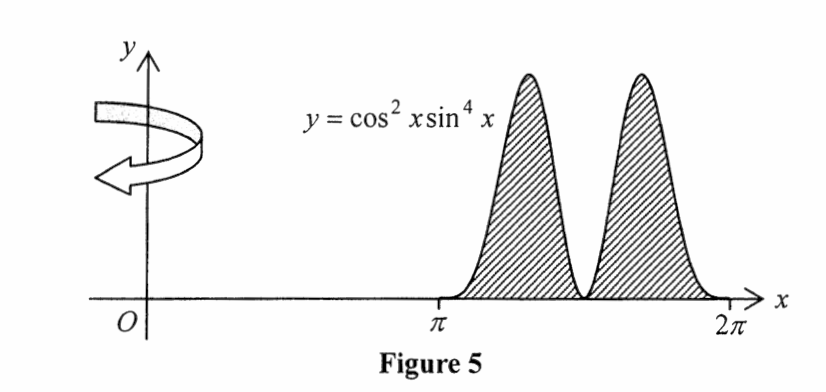
\includegraphics[width = .5\linewidth]{2014Figure5}
			\end{figure}
			(4 marks)
	\end{enumerate}
\end{enumerate}
\end{document}